\documentclass[11pt]{article}
\usepackage[margin=1in]{geometry}
\usepackage{mathpazo}
\usepackage{amsmath,amssymb,amsthm,mathtools}
\usepackage[expansion=false]{microtype}
\usepackage{xcolor}
\usepackage{booktabs,tabularx,array,longtable}
\usepackage{enumitem}
\usepackage{listings}
\usepackage{tikz}
\usetikzlibrary{positioning,arrows.meta,fit,calc,backgrounds}
\usepackage{xurl}
\usepackage[hidelinks]{hyperref}
\usepackage{pdflscape}

\theoremstyle{definition}
\newtheorem{requirement}{Requirement}
\newtheorem{principle}{Principle}
\newtheorem{decision}{Open decision}
\newtheorem{obligation}{Obligation}
\theoremstyle{remark}
\newtheorem{remark}{Remark}

\newcommand{\fl}{f1r3lang}
\newcommand{\Camp}{CampF1R3}
\newcommand{\Kind}{K1ndl1ng}
\newcommand{\MUST}{\textsc{must}}
\newcommand{\MUSTNOT}{\textsc{must not}}
\newcommand{\SHOULD}{\textsc{should}}
\newcommand{\MAY}{\textsc{may}}
\usepackage[htt]{hyphenat}
\newcommand{\code}[1]{\texttt{#1}}
\setlength{\emergencystretch}{3em}

\definecolor{kw}{RGB}{0,0,140}
\definecolor{cm}{RGB}{90,110,90}
\lstdefinelanguage{Rho}{
  keywords={new,in,for,Nil,where,match,if,else,true,false,contract},
  sensitive=true,
  comment=[l]{//},
  morestring=[b]",
}
\lstset{
  language=Rho,
  basicstyle=\ttfamily\small,
  keywordstyle=\color{kw},
  commentstyle=\color{cm}\itshape,
  columns=fullflexible,
  keepspaces=true,
  frame=single,
  framerule=0.3pt,
  rulecolor=\color{black!30},
  xleftmargin=4pt,xrightmargin=4pt,
  aboveskip=6pt,belowskip=6pt,
  breaklines=true,
  literate={<-}{{$\leftarrow$}}1 {<=}{{$\Leftarrow$}}1
}

\title{\textbf{A Browser with \fl{} as its Native Execution Mechanism}\\[4pt]
\large Architecture proposal and review of browser component frameworks\\[6pt]
\normalsize Version 0.2 (draft for review)}
\author{Lucius Gregory Meredith\\
\small CEO, F1R3FLY.io, and Chief Science Officer, F1R3FLY Industries}
\date{28 September 2026}

\begin{document}
\maketitle

\begin{abstract}
\noindent
This proposal designs a web browser in which JavaScript and its execution
environment are replaced by \fl{} (f1r3|@ng), running on a native RSpace inside the
browser client. It first reviews the available browser component frameworks as they
stand in September 2026 --- Electron, the Chromium Embedded Framework, Tauri and
Wry, Servo, Blitz, Ladybird, WebKit and Gecko --- and recommends building on
\textbf{Blitz}, a modular Rust HTML/CSS engine that has no JavaScript engine to
remove, with \textbf{Servo} held in an isolated process for legacy JavaScript pages.
The execution substrate is the existing \Camp{} executive (\Kind{} parser and
normaliser, \Camp{} store, \code{b3ll0ws} interpreter, \code{f1r3x-host}), which is
already dependency-free, WebAssembly-portable, and deliberately
application-agnostic. The architecture then follows from three identifications: a
page is a process, the document is a namespace of unforgeable names, and events are
data on channels. Security becomes capability discipline rather than same-origin
policy, cost accounting becomes a per-page resource budget, deterministic replay
becomes a debugger, and graded where-clauses become the programmable arbiter of
user-interface races. Version~0.2 adds two dimensions. The first makes a
F1R3FLY shard the server: resources are authenticated by content and by consensus
state rather than by the channel they arrive on, which removes substitution by a man in
the middle, and sessions become shared names bound to browser-held keys, which removes
cookies. The second says when to convert between \fl{} resources and standard Web
resources: import pins, export projects, and behaviour never converts. A five-phase development plan, a list of obligations, and the
decisions that need an owner close the document.
\end{abstract}

\tableofcontents

%======================================================================
\section{Summary and recommendation}\label{sec:summary}

The recommended stack, in one line each:

\begin{description}[nosep,leftmargin=1.5em,style=nextline]
\item[Document engine: Blitz.] Its \code{blitz-dom} crate combines Stylo (Firefox's
  CSS engine), Taffy (layout) and Parley (text), with \code{html5ever} for parsing,
  a Vello/wgpu painter, and a winit/AccessKit shell~\cite{blitz}. It has no
  JavaScript engine, so nothing has to be ripped out; the script host is a hole
  waiting to be filled.
\item[Execution: the \Camp{} executive.] \code{k1ndl1ng-parse},
  \code{k1ndl1ng-norm}, \code{campf1r3-core}, \code{b3ll0ws}, \code{f1r3x} and
  \code{f1r3x-host}, unchanged, instantiated once per page. The new code is one
  crate, the \emph{page bridge}, that grounds a page's free names to capabilities
  and translates between channel traffic and DOM mutation.
\item[Legacy web: Servo, out of process.] A quarantined tab type for pages that
  need JavaScript, with no access to \fl{} capabilities except an explicit message
  channel. CEF is the fallback if Servo's compatibility is not sufficient.
\item[Reach: \code{f1r3x-wasm}.] The same \fl{} pages run in unmodified browsers
  through the existing wasm host and a small loader, so authors are not locked out
  of an audience while the native browser matures.
\item[Server: a F1R3FLY shard.] Sites are \code{rho:serve} projects in the
  node's versioned registry, keyed by the publisher's key. Content is addressed by hash,
  bindings are checked against finalized state, and sessions are names bound to
  browser-held keys (Section~\ref{sec:shard}).
\item[Integration: pin and project.] Web resources that \fl{} code depends on are pinned
  by hash; \fl{} resources are projected to the Web, with their hash and a link home,
  for audiences and machines that cannot run them (Section~\ref{sec:integration}).
\end{description}

\noindent
Electron and Tauri are rejected as the base: in both, JavaScript is the application
runtime, so \fl{} could only ever be a guest. The reasons, and the full comparison,
are in Section~\ref{sec:review}.

%======================================================================
\section{Context: what the F1R3FLY codebases already provide}\label{sec:context}

The design leans heavily on work that exists. This section records what was found
in the three repositories on 28 September 2026.

\subsection{\Camp{} (\code{F1R3FLY-io/campf1r3})}

The repository implements a rho executive in roughly 12{,}600 lines of Rust across
eleven crates, with no external dependencies. Every crate except the FFI carries
\code{\#![forbid(unsafe\_code)]}. The pieces that matter here:

\begin{itemize}[nosep]
\item \code{campf1r3-core} is the store: data and waiting continuations at channels,
  with produce, consume and install as single cuts. Its specification requires
  \code{wasm32-unknown-unknown} as a first-class target, requires observable
  counters to be fixed-width so that 32-bit wasm and 64-bit native builds agree bit
  for bit, and forbids \code{tokio}, \code{rayon}, \code{heed} and any C library.
\item Choice is isolated in an oracle $\omega$ with three profiles:
  \code{Free}, \code{Deterministic} (the default; results and the event log are
  bit-identical across targets and thread counts) and \code{Replay} (the store
  accepts only communications matching a loaded log). This is exactly the seam at
  which graded resolution attaches (Section~\ref{sec:graded}).
\item Accounting is hooked at the COMM and nowhere else, through an
  \code{Observer} trait whose \code{Err} aborts the operation atomically.
\item \code{f1r3x-host} is a driver written as a state machine rather than a
  thread: \code{Session::poll(now\_ms)} returns frames, and time is injected. A
  native host calls it from a thread; a page calls it from
  \code{requestAnimationFrame}. Pacing is lockstep or free-running with a bounded
  buffer, as one rule with two bounds.
\item \code{f1r3x-wasm} already runs the executive in a browser tab, without
  \code{wasm-bindgen}, with a working visualiser.
\item \code{k1ndl1ng-norm} produces a normal form with de Bruijn indices and ordered
  parallel components, content-hashed with BLAKE2b-256, so name equality is a byte
  comparison. The deploy path grounds free names by replacing each with an
  unforgeable derived from its identifier.
\end{itemize}

\noindent
The kernel is stratified: K0 is pure rho, K1 adds polyadic communication, joins,
persistence, peek, patterns and \code{new}, and K2 adds \code{where} clauses over the
\code{rho-pure-eval} expression subset, behind a feature flag. The project memo
recorded when the repository was split from Rhobots-in-Space states the constraint
this proposal relies on: \Camp{} must stay application-agnostic so that it can serve
many applications, including a browser via WebAssembly. Nothing in this proposal
adds browser code to that repository.

\subsection{\code{f1r3node-rust}}

The node workspace (\code{node}, \code{casper}, \code{rholang}, \code{rspace++},
\code{rho-pure-eval} and others) is the shard side. Two facts shape the design.
First, \code{rspace++} depends on \code{heed} (LMDB), \code{tokio} and \code{rayon},
so it is not the client RSpace; \Camp{} is. Second, the node exposes an HTTP API
(\code{/api/deploy}, \code{/api/registry/\{uri\}}, \code{/api/blocks}, among others)
and an event stream at \code{/ws/events}, which is sufficient for a first shard
bridge (Section~\ref{sec:shard}). The feature branches
\code{feature/cost-accounting-transpiler}, \code{feature/f1r3lang-mettail-only} and
\code{feature/module-syntax} carry the surface language and its compilation to the
kernel; the browser consumes their output rather than embedding them.

\subsection{The \code{fuzzyware} directory of \code{publications}}

The graded where-clause papers change one thing about the calculus: the
\code{where} clause of a for-comprehension is valued in a commutative semiring
$V$ rather than in the Booleans, and is evaluated per candidate match rather than
per communication~\cite{gradedwhere}. The companion notes instantiate $V$ as
$\mathbb{R}_{\geq 0}$ (probabilistic logic, and the learner's gradient in the
fibre~\cite{gradedpln}) and $\mathbb{C}$ (amplitudes and the Born
rule~\cite{gradedquantum}). The choice-formulae note adds that for idempotent
semirings such as Viterbi $(\max,\times)$ and tropical $(\min,+)$ the clause is
attained by a definable selection function, and that weak fairness is a clause
combinator $\psi \oplus \varepsilon$. For a browser, this is the language in which a
page says how its races are to be arbitrated.

%======================================================================
\section{Goals, non-goals and principles}\label{sec:goals}

\subsection{Goals}
\begin{enumerate}[nosep]
\item \fl{} is the only language a page's behaviour is written in. There is no
  JavaScript engine in the page process.
\item Each page runs against its own RSpace, in the client, with the same semantics
  as the shard's.
\item HTML and CSS rendering are standards-based and reused, not reinvented.
\item A F1R3FLY shard is the server: sites are published to it, and the client authenticates what it receives against it.
\item Every page execution is reproducible from its event log.
\item Desktop first (macOS, Linux, Windows); the same core on mobile and headsets
  later.
\end{enumerate}

\subsection{Non-goals}
\begin{enumerate}[nosep]
\item Running arbitrary JavaScript pages in the native engine. They go to the legacy
  tab (Section~\ref{sec:compat}).
\item Reproducing the Web API surface (\code{window}, \code{fetch}, \code{localStorage})
  under \fl{} names. The design replaces it with capabilities.
\item Consensus in the client. A tab's RSpace is local; the shard remains the place
  where agreement happens.
\item Compiling the full surface language in the browser in version~1. Pages ship
  kernel normal forms (Section~\ref{sec:loading}).
\end{enumerate}

\subsection{Principles}

\begin{principle}[One store, many hosts]
The executive is the same code in the native browser, in the wasm reach tier, on the
Mac server, and behind the Vision Pro client. The browser is a host in the sense of
\code{HOSTING.md}, not a fork.
\end{principle}

\begin{principle}[Names are the only authority]
A page can affect exactly what it holds names for. No ambient global object exists.
\end{principle}

\begin{principle}[The document is data in the namespace]
DOM nodes are reached through names and changed by communication, never by a
foreign-function call that bypasses the store.
\end{principle}

%======================================================================
\section{Review of browser component frameworks}\label{sec:review}

The question each framework was asked is narrow: \emph{can its JavaScript execution
environment be replaced, and what does that cost?} A framework whose value lies in
its JavaScript runtime is disqualified as the base regardless of its other merits.
Status is as of 28 September 2026; sources are listed at the end.

\begin{landscape}
\begin{table}[p]
\centering
\small
\renewcommand{\arraystretch}{1.25}
\newcolumntype{R}[1]{>{\raggedright\arraybackslash}p{#1}}
\begin{tabularx}{\linewidth}{@{}R{2.6cm}R{3.6cm}R{3.9cm}R{2.5cm}R{3.6cm}R{2.1cm}>{\raggedright\arraybackslash}X@{}}
\toprule
Framework & Engine and language & Can JavaScript be replaced? & Rust embedding & Maturity, Sept.\ 2026 & Licence & Role here\\
\midrule
Electron & Chromium and Node.js; C++ & No. V8 and Node \emph{are} the application runtime. & None; Node is the host & Production; a new major every 8 weeks, three supported~\cite{electron} & MIT, Chromium BSD & Rejected\\
CEF & Chromium; C/C++, Rust bindings via \code{cef} crate & No. V8 is wired through Blink's bindings. & Yes (\code{cef}) & Production; tracks Chromium~\cite{cef} & BSD & Fallback for the legacy tab\\
Tauri 2 / Wry & OS webview (WKWebView, WebView2, WebKitGTK); CEF runtime in progress & No. Page logic is JavaScript; Rust is only the backend. & Yes & Production, v2.10~\cite{tauri,tauricef} & MIT/Apache & Rejected as base\\
Servo & Rust; SpiderMonkey for JavaScript & Only by rewriting the \code{script} crate, which holds the DOM and its JS bindings. & Yes (\code{servo} crate, LTS branch) & Pre-1.0; monthly releases, 0.1 LTS in April, 0.5 current~\cite{servolts,servo05} & MPL-2.0 & Legacy tab, isolated\\
\textbf{Blitz} & \textbf{Rust: Stylo, Taffy, Parley, html5ever, Vello} & \textbf{Nothing to replace: it has no JavaScript.} & \textbf{Yes, crate by crate} & \textbf{Beta; renders many no-JS sites}~\cite{blitz} & \textbf{Apache/MIT} & \textbf{Document engine}\\
Ladybird & C++ with a Rust migration; own LibJS & Not a design goal & No & Pre-alpha; public alpha targeted for 2026~\cite{ladybird} & BSD-2 & Watch\\
WebKit (WPE, GTK) & C++; JavaScriptCore & No & C API only & Production & LGPL/BSD & Rejected\\
Gecko / GeckoView & C++ and Rust; SpiderMonkey & No & Android only & Production & MPL-2.0 & Rejected\\
Stock browser + \code{f1r3x-wasm} & Host browser; \Camp{} as wasm & JavaScript stays as a thin loader & n/a & Working today in \code{campf1r3} & Apache-2.0 & Reach tier\\
\bottomrule
\end{tabularx}
\caption{Browser component frameworks against the one question that matters here.}
\label{tab:frameworks}
\end{table}
\end{landscape}

\subsection{Electron}
Electron embeds Chromium and Node.js into one binary so that a single JavaScript
codebase can drive a desktop application~\cite{electron}. That is its entire value
proposition, and it is the opposite of this project's. Replacing V8 would mean
maintaining a Chromium fork with Blink's bindings layer rewritten, rebased every
eight weeks as Electron tracks Chromium majors. The best that could be done without
that is to run \Camp{} as wasm inside Electron's renderer, which is the reach tier
with a heavier wrapper. Electron is rejected.

\subsection{Chromium Embedded Framework}
CEF embeds a complete Chromium and is the industry default for putting a real
browser inside an application; Rust bindings are maintained under the Tauri
organisation~\cite{cef}. Its JavaScript engine is equally unremovable. Its merit
here is compatibility: if the legacy tab must render the modern JavaScript web at
Chromium fidelity, CEF in a separate process is the dependable answer, at a cost
reported by one embedder as a runtime of about 170\,MB~\cite{atrium}.

\subsection{Tauri 2 and Wry}
Tauri builds applications from a Rust backend and a web frontend rendered by the
operating system's webview, and an official CEF runtime is being built in its
repository~\cite{tauricef}. Tauri is attractive for application shells, but in every
configuration the page's behaviour is JavaScript and Rust is reached through IPC. A
Tauri application could host \Camp{} natively in its Rust half and give pages a
bridge to it, but then \fl{} is an RPC target of JavaScript, which inverts the goal.
Tauri is rejected as the base. Two of its crates (\code{muda} for menus,
\code{tao} or \code{winit} for windows) are used by Blitz's shell anyway.

\subsection{Servo}
Servo is a Rust engine under Linux Foundation Europe, now published as a crate with
a WebView embedding API and a long-term-support branch every six months, supported
for nine months~\cite{servolts}. Monthly releases continue, and 0.5 brought faster
text rendering and wider site compatibility~\cite{servo05}. Architecturally it is the
closest mainstream engine to what is wanted: Rust throughout, parallel styling, a
clean embedder boundary. But its \code{script} crate --- the DOM implementation and
the event loop --- is generated from WebIDL onto SpiderMonkey's garbage-collected
object model. Removing JavaScript means replacing \code{script}, which is the largest
and most web-compatibility-sensitive part of the engine. Servo is therefore the right
engine for the legacy tab, where JavaScript is wanted, and the wrong one to hollow
out.

\subsection{Blitz}
Blitz is a modular HTML/CSS engine from Dioxus Labs, in beta, that renders many
no-JavaScript sites and is usable for applications by early adopters~\cite{blitz}.
It is assembled from the same parts as Servo's style system (Stylo, html5ever) plus
Taffy for box layout, Parley for text, AccessKit for accessibility and an
\code{anyrender} abstraction over Vello and other painters. Its authors state that
it renders HTML and CSS and deliberately does \emph{not} ship a JavaScript engine,
local storage, WebSockets and similar features, leaving them to native crates.
Interactivity today comes from Dioxus Native, which drives \code{blitz-dom}'s tree
from Rust. That is precisely the seam \fl{} needs: replace the Dioxus virtual DOM
with the page bridge, and the executive drives the document. The risks are maturity
and the size of the team; they are addressed in Section~\ref{sec:risks}.

\subsection{Ladybird}
Ladybird is an independent engine built from scratch by a non-profit, reporting over
two million passing Web Platform Test subtests and a Rust rewrite of its JavaScript
front end in February 2026, with a public alpha targeted for 2026~\cite{ladybird}.
It is a browser, not a component; it has no embedding story and its JavaScript engine
is one of its central investments. It is worth watching as a future legacy-tab engine
and as evidence that a new engine can reach real compatibility, but it is not a base.

\subsection{WebKit and Gecko}
Both are production engines whose JavaScript engines are woven through their DOM
implementations, with C and C++ embedding surfaces (WPE, GeckoView on Android). They
offer nothing over CEF for the legacy role and nothing at all for the native one.

\subsection{The reach tier: \Camp{} in a stock browser}
\code{f1r3x-wasm} already runs the executive inside an ordinary tab, driven from the
page's animation loop. A small loader plus a DOM bridge written against the host
browser's DOM gives \fl{} pages an audience on every browser today. JavaScript
remains present as the host's glue, so this tier does not meet Goal~1, but it shares
every line of the executive with the native browser, which makes it the natural
bootstrap and the natural test oracle.

%======================================================================
\section{Recommendation}\label{sec:rec}

\begin{requirement}[Framework choice]
The native browser \MUST{} use Blitz (\code{blitz-dom}, \code{blitz-html},
\code{blitz-paint}, \code{blitz-net}, \code{blitz-shell}) as its document engine and
the \Camp{} executive as its only execution mechanism. Legacy JavaScript pages
\SHOULD{} be rendered by Servo in a separate process, with CEF as the fallback. The
reach tier \SHOULD{} be delivered from \code{f1r3x-wasm}.
\end{requirement}

\noindent
Four reasons, in order of weight.

\begin{enumerate}
\item \textbf{Subtraction versus addition.} Every other engine requires removing a
  JavaScript engine that its DOM was designed around. Blitz requires adding a script
  host to a DOM designed to be driven from outside. Addition is bounded; subtraction
  from a browser engine is not.
\item \textbf{One language, one toolchain.} Blitz, \Camp{} and the node are all
  Rust, with permissive or file-level-copyleft licences (Apache, MIT, MPL-2.0 for
  Stylo) compatible with F1R3FLY's Apache-2.0 practice. There is no C++ build, no
  Chromium checkout and no rebasing treadmill.
\item \textbf{Alignment with the store's discipline.} \Camp{} is small,
  dependency-free and portable by requirement; Blitz is modular by design and
  already builds for wasm (its repository carries a wasm how-to). Both can be
  pinned and vendored, and both can run on a headset.
\item \textbf{Shared lineage with the legacy engine.} Blitz and Servo share Stylo
  and html5ever, so CSS behaves the same in native and legacy tabs, and fixes
  upstream benefit both.
\end{enumerate}

\begin{remark}
Choosing Blitz is choosing to own more of the engine than an Electron application
would. That is intended: the point of the project is that the execution environment
of the web is the thing being changed, and it cannot be changed from inside a
framework whose purpose is to preserve it.
\end{remark}

%======================================================================
\section{Architecture}\label{sec:arch}

The browser is three kinds of operating-system process and one remote party
(Figure~\ref{fig:arch}). The \emph{browser process} owns windows, the user's keys,
the network and the capability broker. Each \emph{page process} holds one site's
tabs: a Blitz document per tab and one \Camp{} executive per tab, joined by the page
bridge. A \emph{legacy process}, started only when needed, runs Servo for pages that
require JavaScript. The \emph{shard} is reached through the browser process, never
directly from a page.

\begin{figure}[!htb]
\centering
\resizebox{\linewidth}{!}{%
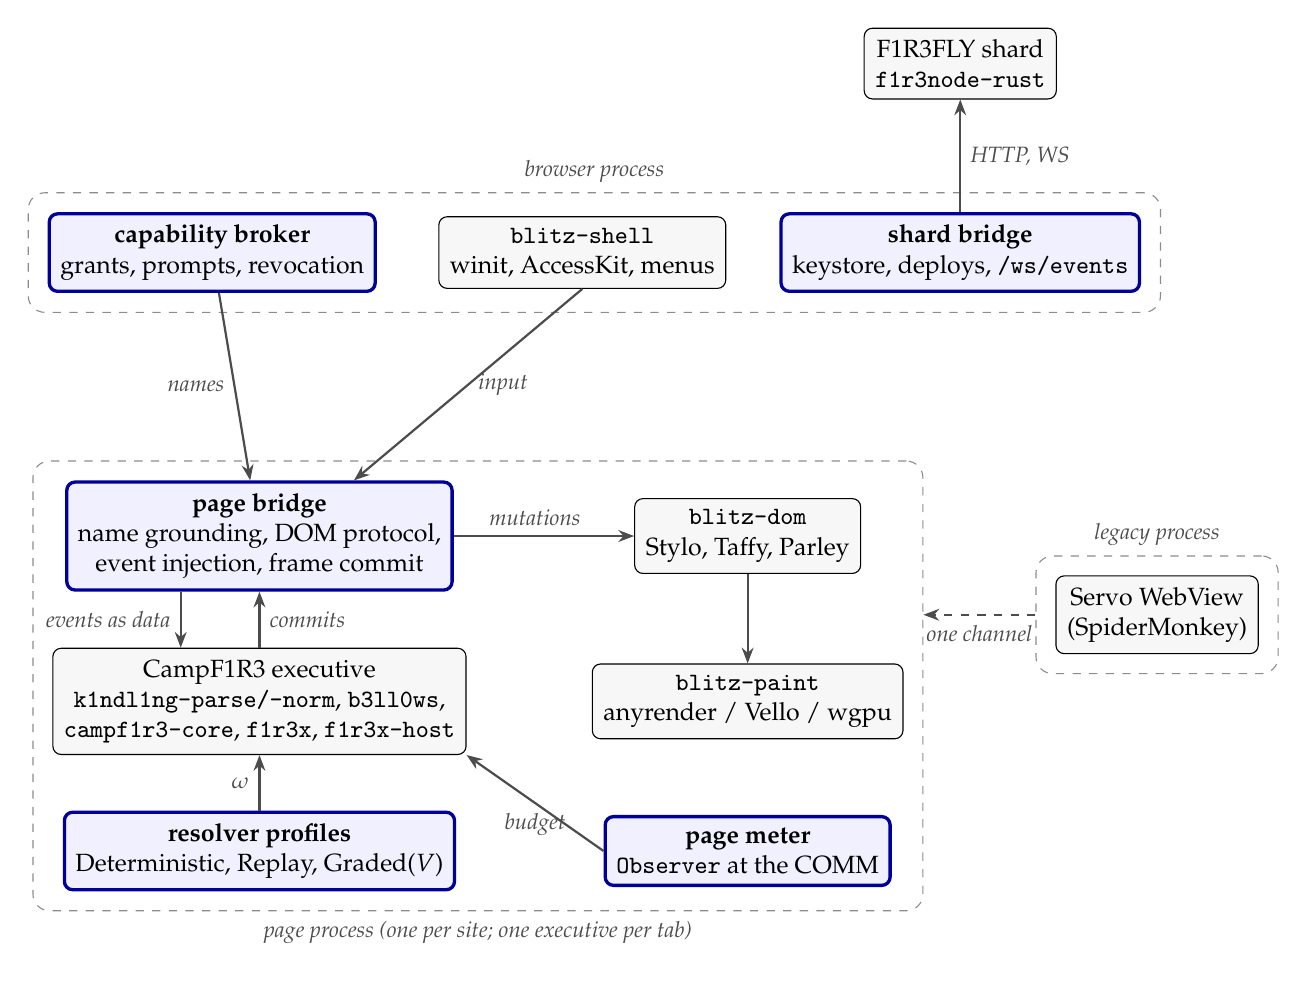
\begin{tikzpicture}[
  font=\small,
  box/.style={draw, rounded corners=3pt, align=center, minimum height=8mm, inner sep=4pt},
  new/.style={box, draw=blue!60!black, fill=blue!6, very thick},
  reuse/.style={box, fill=black!3},
  proc/.style={draw=black!45, dashed, rounded corners=6pt, inner sep=7pt},
  arr/.style={-{Stealth[length=2mm]}, thick, black!70},
  lbl/.style={font=\footnotesize\itshape, black!70}
]
% Page process
\node[new]   (bridge) at (0,0) {\textbf{page bridge}\\ name grounding, DOM protocol,\\ event injection, frame commit};
\node[reuse] (exec)   at (0,-2.1) {\Camp{} executive\\ \code{k1ndl1ng-parse/-norm}, \code{b3ll0ws},\\ \code{campf1r3-core}, \code{f1r3x}, \code{f1r3x-host}};
\node[reuse] (dom)    at (6.2,0) {\code{blitz-dom}\\ Stylo, Taffy, Parley};
\node[reuse] (paint)  at (6.2,-2.1) {\code{blitz-paint}\\ anyrender / Vello / wgpu};
\node[new]   (resolver) at (0,-4.0) {\textbf{resolver profiles}\\ Deterministic, Replay, Graded($V$)};
\node[new]   (meter) at (6.2,-4.0) {\textbf{page meter}\\ \code{Observer} at the COMM};
\draw[arr] (bridge) -- node[lbl,above,pos=0.45]{mutations} (dom);
\draw[arr] (dom) -- (paint);
\draw[arr] (exec) -- node[lbl,right]{commits} (bridge);
\draw[arr] ([xshift=-10mm]bridge.south) -- node[lbl,left]{events as data} ([xshift=-10mm]exec.north);
\draw[arr] (resolver) -- node[lbl,left]{$\omega$} (exec);
\draw[arr] (meter.west) -- node[lbl,below]{budget} (exec.south east);
\begin{scope}[on background layer]
\node[proc, fit=(bridge)(exec)(dom)(paint)(resolver)(meter), label={[lbl]below:page process (one per site; one executive per tab)}] (pp) {};
\end{scope}
% Browser process
\node[new]   (broker) at (-0.6,3.6) {\textbf{capability broker}\\ grants, prompts, revocation};
\node[reuse] (shell)  at (4.1,3.6) {\code{blitz-shell}\\ winit, AccessKit, menus};
\node[new]   (sbridge) at (8.9,3.6) {\textbf{shard bridge}\\ keystore, deploys, \code{/ws/events}};
\begin{scope}[on background layer]
\node[proc, fit=(broker)(shell)(sbridge), label={[lbl]above:browser process}] (bp) {};
\end{scope}
\draw[arr] (broker) -- node[lbl,left]{names} (bridge);
\draw[arr] (shell.south) -- node[lbl,right]{input} ([xshift=12mm]bridge.north);
% Legacy and shard
\node[reuse] (servo) at (11.4,-1.0) {Servo WebView\\ (SpiderMonkey)};
\begin{scope}[on background layer]
\node[proc, fit=(servo), label={[lbl]above:legacy process}] (lp) {};
\end{scope}
\node[reuse] (shard) at (8.9,6.0) {F1R3FLY shard\\ \code{f1r3node-rust}};
\draw[arr] (sbridge) -- node[lbl,right]{HTTP, WS} (shard);
\draw[arr, dashed] (lp.west) -- node[lbl,below]{one channel} (pp.east|-lp.west);
\end{tikzpicture}}
\caption{Processes and components. Heavy boxes are new code; light boxes are reused
unchanged from \code{campf1r3} and Blitz. The executive never calls the DOM; it
communicates, and the bridge turns communications into mutations.}
\label{fig:arch}
\end{figure}

\subsection{What is new, and what is not}

The new code is four components, all outside the \code{campf1r3} repository:

\begin{enumerate}[nosep]
\item \textbf{The page bridge} (\S\ref{sec:exec}): grounds free names, speaks the
  DOM protocol, injects events, and commits a round's mutations to \code{blitz-dom}
  once per frame.
\item \textbf{The capability broker}: decides which names a page receives, asks the
  user where a grant needs consent, and can revoke by killing a forwarder.
\item \textbf{The shard bridge} (\S\ref{sec:shard}): holds keys, signs deploys,
  proxies registry and data-at-name reads, and turns the node's event stream into
  produces on local channels.
\item \textbf{The resolver and meter profiles} (\S\ref{sec:graded},
  \S\ref{sec:cost}): a Graded oracle for \Camp{} and a per-page accounting observer.
\end{enumerate}

\noindent
Everything else is reused. In particular the executive is linked natively in the page
process for speed and multi-core stores, and the \emph{same} crates are what the reach
tier ships as wasm.

\subsection{Process model}

\begin{requirement}[Isolation]
A page process \MUST{} hold pages of one site only. The legacy process \MUSTNOT{}
hold any name granted to a \fl{} page, and \MUST{} communicate with page processes
only through a single broker-mediated channel carrying ground data.
\end{requirement}

\noindent
Rust's memory safety and \Camp{}'s \code{forbid(unsafe\_code)} remove the most common
reason browsers isolate renderers, but process-per-site is kept because it is also
the unit of crash containment, of resource limits enforced by the operating system,
and of the legacy engine's quarantine. As defence in depth, the executive
\MAY{} additionally run as \code{wasm32} inside the page process under a wasm
runtime, since it already builds for that target; whether the cost is worth it is
Obligation~\ref{ob:wasmdepth}.

%======================================================================
\section{Execution model}\label{sec:exec}

\subsection{A page is a process}\label{sec:loading}

A \fl{} page is an HTML document whose behaviour is given by processes, carried as
\begin{lstlisting}
<script type="application/f1r3lang" src="counter.knf"
        integrity="blake2b-256:..."></script>
\end{lstlisting}
or inline. The loader accepts kernel text (parsed at the level the page declares,
K1 by default, K2 when graded clauses are used) or an encoded normal form. Because
\code{k1ndl1ng-norm} content-hashes the normal form, the integrity attribute is not an
add-on: it \emph{is} the program's identity, it keys the parse cache, and two pages
that load the same process share one cached plan in \code{b3ll0ws}.

The surface language is compiled to the kernel ahead of time by the \fl{} toolchain,
as TypeScript is compiled to JavaScript. This keeps the compiler, the DDL and the
cost-accounting transpiler out of the browser's trusted base in version~1 and makes
\code{.knf} the web's unit of shipped behaviour. Compiling in the browser is
Decision~\ref{dec:compile}.

\subsection{Imports are free names}

A page's process is closed except for its free names, and \Camp{}'s deploy path
already grounds every free name to an unforgeable derived from its identifier. The
browser changes only \emph{what the grounding is derived from}: the capability
broker supplies, for each free identifier the page uses, either a granted system
name or a dead channel. The page's import list is therefore computable from its
normal form before a single reduction, which lets the browser show the user what a
page will ask for before it runs.

\begin{center}
\begin{tabularx}{\linewidth}{@{}lX@{}}
\toprule
Free name & Granted capability\\
\midrule
\code{doc} & the document root (Section~\ref{sec:dom})\\
\code{net} & fetch, restricted to the page's origin unless widened by grant\\
\code{store} & per-origin persistent space: a \Camp{} checkpoint saved by the browser\\
\code{clock} & frame ticks and timers\\
\code{log} & the developer console\\
\code{shard} & the shard bridge, only after an explicit user grant\\
\bottomrule
\end{tabularx}
\end{center}

\subsection{The document is a namespace}\label{sec:dom}

Every element the page can reach is represented by an unforgeable name minted by the
bridge. The bridge keeps a table from those names to \code{blitz-dom} node ids;
the table never leaves the bridge. A page receives names only by asking for them on a
name it already holds.

\begin{principle}[Attenuation is the tree]
Queries on an element's name return only that element's descendants. Holding a
subtree's name therefore grants exactly that subtree, and handing a component a
container's name confines it to the container.
\end{principle}

\noindent
This is the object-capability discipline, and here it costs nothing: it is what
unforgeability already means. A third-party widget embedded in a page gets the name of
its slot and cannot read the rest of the document, which today requires iframes and
cross-origin machinery.

The protocol on an element's name is a small set of messages, each carrying a return
channel where a reply is expected: \code{query} and \code{query1} (selectors, answered
with names), \code{get} and \code{set} for properties and attributes, \code{class},
\code{append}, \code{replace} and \code{remove} with HTML fragments or structured terms,
and \code{listen} to subscribe a channel to an event type. Reads are answered from the
committed document, so a page never observes a half-applied frame.

\subsection{Events are data on channels}

\code{listen} installs a forwarder: each occurrence of the event is produced as a
datum on the page's channel. Handlers are ordinary receipts, persistent when they
should fire repeatedly. A lamp that toggles on click, in surface syntax:

\begin{lstlisting}
new found, clicks, on, off in {
  doc!("query1", "#lamp", *found) |
  for (lamp <- found) {
    lamp!("listen", "click", *clicks) |
    off!(Nil) |
    for (_ <= clicks & _ <- off) { lamp!("class", "lit") | on!(Nil) } |
    for (_ <= clicks & _ <- on)  { lamp!("class", "")    | off!(Nil) }
  }
}
\end{lstlisting}

\noindent
There is no state variable and no callback: the state is which token exists, and the
join is the state machine. Because exactly one token exists, the two handlers never
race. Bubbling and default actions are implemented by the bridge, not the page:
an event's datum carries a reply name, a handler that wants to stop propagation or
prevent the default says so on it, and the bridge applies the default after a
deadline if no handler has answered.

\subsection{The frame is the unit of commit}

\code{f1r3x-host} already separates \emph{what} reduces from \emph{when} a decided
commit is released. The page process drives \code{Session::poll(now)} from the shell's
frame callback; a round's commits carry DOM messages; the bridge applies them to
\code{blitz-dom} as one batch; Stylo restyles, Taffy lays out, and the painter
draws. The host's two pacing modes map directly: \emph{free-running} for ordinary
pages, with the bounded buffer providing back-pressure when a page produces faster
than frames can show; \emph{lockstep} for the debugger, where the user steps one round
at a time and the document updates with each.

\begin{requirement}[Frame atomicity]
Mutations produced within one admitted round \MUST{} be applied to the document
together, and style and layout \MUST{} be computed only between rounds.
\end{requirement}

\subsection{Determinism, replay and the debugger}

In the \code{Deterministic} profile, \Camp{}'s results and event log are
bit-identical across targets and thread counts. A page's run is then a function of
its normal form and the sequence of events injected at its apertures (user input,
network replies, timer ticks). The browser records that sequence with the log. Three
features follow at no further semantic cost:

\begin{itemize}[nosep]
\item \textbf{Bug reports are replays.} A report is the page hash, the grants and the
  log; the developer re-runs it in the \code{Replay} profile and sees the same run.
\item \textbf{Time travel.} \Camp{}'s soft checkpoints let the debugger step back as
  well as forward.
\item \textbf{A live view of the space.} \code{k1ndl1ng-norm::json} and the host's
  scene frames already describe the store for a visualiser; the same vocabulary serves
  a devtools pane, and the Rhobots headset client can attach to a page as easily as to
  the Mac server.
\end{itemize}

\subsection{Cost accounting as a page budget}\label{sec:cost}

\Camp{} hooks accounting at the COMM through an \code{Observer} that may abort. The
browser installs a \emph{page meter}: an observer debiting a per-tab budget replenished
per frame, with a larger allowance for the foreground tab. A page that exhausts its
budget stops making progress without stopping the browser, and the user sees why.
This replaces the ``page is not responding'' heuristic with an exact quantity, bounds
the damage from runaway or hostile code (including in-page mining), and uses the same
cost model the shard charges for, so a developer can predict a deploy's cost from a
local run.

\subsection{Graded where-clauses arbitrate the page's races}\label{sec:graded}

Interfaces are full of races: two handlers for one keystroke, a stale network reply
against a fresh one, an animation against an interaction. In JavaScript these are
settled by event-loop ordering that the programmer does not control. In \fl{} they
are settled by the resolver, and the graded where-clause is the syntax in which the
page arranges it. \Camp{} already isolates choice in the oracle $\omega$; the proposal
adds a \code{Graded} profile that evaluates each candidate's clause in the page's
declared semiring $V$ and selects accordingly.

\begin{center}
\begin{tabularx}{\linewidth}{@{}p{3.1cm}p{3.6cm}X@{}}
\toprule
Semiring $V$ & Resolver & Use in a page\\
\midrule
Booleans & any enabled candidate & today's rholang guards\\
Viterbi $(\max,\times)$ & argmax, attained exactly & priorities: the autocomplete handler outranks the fallback, deterministically\\
tropical $(\min,+)$ & least cost, attained exactly & choose the cheapest source: cached, local, or network\\
$\mathbb{R}_{\geq 0}$ & sample the normalised clause & randomised layouts, experiments, load spreading\\
$\mathbb{R}_{\geq 0}$ with learning & sample, then update in the fibre & interfaces that adapt to the user locally, without a server\\
\bottomrule
\end{tabularx}
\end{center}

\noindent
Two results from the choice-formulae note are directly useful. First, weak fairness
is the combinator $\psi\oplus\varepsilon$: a page, or the browser on the page's behalf,
can guarantee that no persistently enabled handler starves. Second, strength enters a
program only at \emph{apertures} or through reflection, so a static pass over a page's
normal form bounds the choice strength of everything in its interior; the browser can
refuse, or run in a restricted profile, a page whose interior exceeds a declared
ceiling. The quantum instance $V=\mathbb{C}$ is out of scope for the browser; the
resolver seam is where it would go.

\begin{requirement}[Graded resolution is opt-in]
A page that does not declare a semiring \MUST{} run in the \code{Deterministic}
profile. Replay of a graded page \MUST{} record the resolver's selections in the log,
so that sampled runs are reproducible.
\end{requirement}

%======================================================================
\section{The shard as the server}\label{sec:shard}

\subsection{What the Web authenticates, and what it does not}

The Web authenticates \emph{channels}. TLS proves that the bytes arrived from a
party holding a certificate for a hostname; it says nothing about whether those bytes
are the ones the author published. Every party that terminates TLS on the author's
behalf --- a CDN edge, a load balancer, a compromised origin, a hosting provider, a
misissued certificate --- can substitute a resource, and the client cannot tell.
Subresource Integrity covers only subresources named by a document that was itself
trusted because of its channel. The root document, and every dynamic response, is
authenticated by location alone. Sessions compound the problem: a cookie is a bearer
token attached ambiently to every request to its domain, so whoever copies it is the
user, and any page that can cause a request to that domain speaks with the user's
authority.

\begin{principle}[Authenticate content, not channels]
The browser establishes the integrity of a resource from the resource and the
shard's agreed state, never from the connection it arrived on. Transport encryption
remains, for confidentiality; it stops being load-bearing for integrity.
\end{principle}

\noindent
Under this principle, a man in the middle can still withhold, delay or observe
traffic. It can no longer substitute. The rest of this section shows how each kind of
resource reaches that standard.

\subsection{Three kinds of resource}

\begin{center}
\begin{tabularx}{\linewidth}{@{}p{3.0cm}p{4.2cm}X@{}}
\toprule
Kind & Identity & How the client authenticates it\\
\midrule
Immutable content (code, documents, media) & its hash: the \Kind{} normal-form hash for processes, BLAKE2b-256 of the bytes for blobs & recompute the hash; any transport will do\\
Mutable binding (``the current version of this site'') & a versioned-registry name: publisher key, project, version range & the binding is shard state, established by consensus and checked against a finalized block\\
Dynamic response (the result of a computation) & a deploy, or a session message (\S\ref{sec:sessions}) & re-execute locally in the \code{Replay} profile, or accept an attested result at a stated assurance level\\
\bottomrule
\end{tabularx}
\end{center}

\paragraph{Immutable content is self-certifying.}
A page is named by the hash of its normal form, and a blob by the hash of its bytes.
The client recomputes the hash on receipt, so it can fetch from the shard, from a
mirror, from a peer, or from an ordinary CDN without trusting any of them. This turns
existing caching infrastructure into an untrusted transport, which is what it should
have been: hash-addressed resources never go stale, so they can be cached forever at
every layer. Large blobs \SHOULD{} be kept out of RSpace; the shard stores their hashes
in bindings, and the bytes live in any content-addressed store.

\paragraph{Mutable bindings are consensus state.}
\code{f1r3node-rust} already carries the mechanism. Its versioned registry
(\code{casper/src/main/resources/VersionedRegistry.rho}) implements names of the form
\[
\code{rho:serve:}\langle\mathit{service\ ver}\rangle\code{:}\langle\mathit{pub\ key}\rangle\code{:}\langle\mathit{project}\rangle\code{:}\langle\mathit{project\ ver}\rangle
\]
with semver resolution, deprecation, and notify channels. Its mutators take the
publisher's key from the \emph{authenticated} deployer identity, so ``nothing an
attacker can send on the wire lets them mutate someone else's entries'', as the
contract's own commentary puts it. A website is then a \code{rho:serve} project: the
publisher's key is the site's identity, a version is a release, deprecation is how a
vulnerable release is withdrawn, and the notify channel is how clients learn of it.
DNS and certificate authorities disappear from the integrity path.

The client must still know that the binding it was shown is the agreed one. Blocks
carry a \code{post\_state\_hash} over \code{rspace++}'s history, which is a radix trie
hashed with BLAKE2b-256, and the node's HTTP API answers \code{is-finalized} and
\code{last-finalized-block} queries. What is missing is an endpoint returning an
\emph{inclusion proof}: the trie path from a registry entry to a finalized block's
post-state hash. With it, the browser becomes a light client: it checks the block's
validator signatures against a known bonded set and the path against the hash, and
trusts no node. Without it, the browser falls back to asking several independent nodes
and requiring agreement. This is Obligation~\ref{ob:proofs}.

\paragraph{Freshness.} A valid but old binding is the one substitution content
addressing does not prevent: an attacker can replay a superseded, correctly signed
state. The browser therefore records, per publisher, the highest finalized block at
which it has seen a binding, rejects proofs from older blocks, and subscribes to the
notify channel of every project it has open.

\subsection{Dynamic responses and the assurance ladder}

A dynamic response in this architecture is the result of running a process against
shard state. Because the client holds the same executive, it can in principle
recompute any result whose inputs it can obtain with proofs. That gives a ladder of
assurance, and the browser shows the user which rung a response stands on.

\begin{enumerate}[nosep]
\item \textbf{Node-attested.} An exploratory deploy (read-only; the node bounds its
  concurrency, phlogiston and time) answered and signed by one node.
  Trust: that node.
\item \textbf{Quorum-attested.} The same query answered identically by $k$ of $n$
  independent nodes. Trust: fewer than $k$ colluding.
\item \textbf{Proof-carrying.} The result is data at a name in a finalized post-state,
  delivered with an inclusion proof. Trust: the bonded validator set.
\item \textbf{Re-executed.} The client fetches the process by hash and the state it
  reads with proofs, and replays it locally in the \code{Replay} or
  \code{Deterministic} profile. Trust: the client's own executive.
\end{enumerate}

\noindent
Rung~4 is available only because the client and the shard share a semantics; it
depends on \Camp{} and \code{rspace++} agreeing, which is Obligation~\ref{ob:replay}.

\subsection{Sessions without cookies}\label{sec:sessions}

In \fl{} a session is not an identifier attached to requests. It is a name that two
parties hold and nobody else does:

\begin{lstlisting}
// client, in the page
new session, ack in {
  svc!("open", *session, *ack) |
  for (_ <- ack) { session!("inbox", *ack) | for (@items <- ack) { ... } }
}

// service, published under rho:serve:...
contract svc(@"open", session, ack) = {
  ack!(Nil) |
  for (@"inbox", ret <= session) { ... ret!(items) }
}
\end{lstlisting}

\noindent
Every property cookies were invented to approximate, and every attack they enable,
changes character:

\begin{description}[leftmargin=1.5em,style=nextline]
\item[No ambient authority, so no cross-site request forgery.] A request carries
  authority only because it is sent on the session name. Another page, even one open
  in the next tab, does not hold that name and cannot cause a send on it.
\item[No bearer token to steal.] There is no string whose possession is identity;
  within a runtime the name is unforgeable, and across the network it is bound to a key
  that pages never see (below).
\item[No script to exfiltrate it.] There is no JavaScript, and a third-party component
  holds only the names it was granted.
\item[No tracking side-channel.] Nothing is attached to requests by default, so there
  is no third-party cookie to disable.
\item[The session is visible and killable.] It is a continuation in a store. Ending it
  is consuming the name or revoking its key; the browser can list a tab's open
  sessions as it lists its grants.
\item[Its protocol can be typed.] A session is a channel with a behaviour, so the
  linear fragment and the spatial-behavioural logics already in the programme apply:
  ``this session may be used once'', ``this session answers \code{inbox} before it
  answers \code{send}'' become checkable properties rather than server conventions.
\end{description}

\paragraph{Realising unforgeability across the network.}
Unforgeable names are a property of one runtime. Between the browser and the shard
the name must be realised cryptographically, and the node already has the primitive:
deploys are signed, and a contract can read the authenticated deployer's key through
\code{rho:deploy:data} and \code{rho:system:deployerId:ops}, exactly as the versioned
registry does. The session is therefore opened with a fresh key pair generated by the
browser's keystore. The service keys the session's channel by that public key, and
accepts a message on it only from a deploy signed by the matching private key. Replay
of a captured request is refused because \code{DeployData} carries a timestamp,
\code{validAfterBlockNumber} and an optional \code{expiration\_timestamp} under the
signature. The page holds the session \emph{name}; the browser holds the \emph{key}.
Closing the tab can destroy the key, which ends the session irrevocably.

\subsection{Three server tiers}

A deploy costs phlogiston and waits for consensus, which is right for a purchase or a
vote and wrong for every keystroke of a chat. The design therefore has three tiers, and
a session can span them.

\begin{center}
\begin{tabularx}{\linewidth}{@{}p{2.6cm}p{3.8cm}p{3.1cm}X@{}}
\toprule
Tier & Runs where & Latency & Integrity\\
\midrule
Client & the tab's \Camp{} executive & a frame & the user's own executive\\
Session host & a \Camp{} executive beside a node, reached over WebSocket (\code{f1r3x-serve}, whose sessions already outlive sockets) & a round trip & attested by the host; auditable later by replay of a log whose hash is anchored on the shard\\
Shard & \code{f1r3node-rust} consensus & finalization & the bonded validator set\\
\bottomrule
\end{tabularx}
\end{center}

\noindent
The session host runs in the \code{Deterministic} profile and periodically deploys the
hash of its event log to the shard. Nobody need trust it in the moment to hold it to
account afterwards: any party with the log replays it and compares hashes. Interactive
traffic lives on the session host; commitments that matter move to the shard.

\subsection{Confidentiality}

Integrity is gained; confidentiality is not automatic. Shard state is replicated to
every validator and readable by anyone who can query a node, so session content
committed there in clear is public. Private sessions \MUST{} encrypt payloads end to
end under keys derived from the session keys, or keep private content on the session
host and commit only hashes. Transport encryption continues to protect traffic in
flight. The choice between these is Decision~\ref{dec:privacy}.

\subsection{What remains trusted}

Honesty about the residue: the browser binary and its update channel; the initial
bonded-validator set or a checkpoint of it (the light client's root of trust, taken
once, like a CA bundle but for one shard); the user's keystore; the user interface
that shows grants, assurance levels and deploy costs; and availability, since a
network attacker can still withhold. Traffic analysis is untouched.

%======================================================================
\section{Security model}\label{sec:security}

\begin{description}[leftmargin=1.5em,style=nextline]
\item[Integrity comes from content and consensus.] See Section~\ref{sec:shard}: hashes
  for immutable resources, finalized registry state for bindings, and a stated assurance
  level for dynamic responses.
\item[Capabilities replace the same-origin policy.] A page has no ambient authority:
  no global object, no cookie jar it can read, no network beyond what its \code{net}
  name permits. Cross-origin cooperation is name passing, deliberately.
\item[Grants are visible before execution.] Imports are free names in a normal form,
  so the browser knows a page's full requested authority at load time.
\item[Reflection is code mobility.] Receiving a quoted process and dropping it
  (\code{*y}) runs code that arrived as data --- the rho analogue of \code{eval}. The
  choice-formulae note shows the same construct carries choice strength into an
  interior that was checked without it. The browser therefore meters dropped code under
  the receiving page's budget and, for graded pages, enforces the declared ceiling on
  drops (the stratified where of that note).
\item[Unforgeability is authority, not ownership.] A granted name can be copied to
  another process the page controls; the review of the quantum graded-where paper made
  the same distinction. Revocation is therefore by forwarder: the broker grants a
  proxy name it can sever, never the underlying system name.
\item[The legacy tab is a different trust domain.] It gets no names; it talks to
  \fl{} pages only through one channel of ground data mediated by the broker.
\item[Memory safety.] The page process contains Rust code only; \Camp{} forbids
  \code{unsafe} outside its FFI, which the native browser does not use.
\end{description}

%======================================================================
\section{Compatibility with the JavaScript web}\label{sec:compat}

The browser serves four kinds of content, and says which kind a tab holds.

\begin{enumerate}
\item \textbf{Native \fl{} pages}, rendered by Blitz and driven by the executive.
\item \textbf{Static HTML and CSS} without scripts, rendered natively by Blitz, which
  already handles many such sites. Documentation, articles and much of the long tail of
  the web fall here.
\item \textbf{JavaScript pages}, opened in the legacy process under Servo (or CEF),
  visibly marked, with no access to \fl{} capabilities.
\item \textbf{Mixed pages} in the reach tier: \fl{} pages served to stock browsers run
  under \code{f1r3x-wasm} with a small loader, so one page serves both audiences.
\end{enumerate}

\noindent
WebAssembly modules are a possible later addition as foreign processes: a module
instantiated by the browser, exposed to the page as a name, called by communication.
This keeps computation-heavy libraries available without reintroducing a JavaScript
host. It is not in the plan below.

%======================================================================
\section{Integration with existing web infrastructure}\label{sec:integration}

The greenfield design is only useful if it meets the Web where the Web already is.
The question is when to convert. A \fl{} resource is content-addressed,
capability-scoped and replayable; a Web resource is location-addressed, ambiently
authorised and opaque. Conversion in either direction changes which of those
properties hold, so the decision is about which properties someone downstream will
actually use.

\subsection{Four rules}

\begin{principle}[Import pins, export projects]
Bringing a Web resource in fixes it: fetch, hash, and from then on refer to it by hash.
Sending a \fl{} resource out produces a \emph{projection}: a Web rendering that keeps
what the Web can carry and drops the rest.
\end{principle}

\begin{principle}[Convert data and bindings, never behaviour]
Documents, media, datasets and name bindings convert in both directions. JavaScript
applications do not become \fl{} processes, and \fl{} processes do not become
JavaScript; behaviour crosses only by running in its own engine (the legacy tab one
way, \code{f1r3x-wasm} the other).
\end{principle}

\begin{principle}[Every projection points home]
An exported resource carries the address it was projected from, so a native client that
meets the projection can upgrade to the original, the way a client follows
\code{Alt-Svc} to a better transport.
\end{principle}

\begin{principle}[Convert where a guarantee stops being used]
Pin a Web resource when \fl{} code will depend on it, because replay needs fixed
inputs. Project a \fl{} resource when its consumer cannot check what the projection
drops. Otherwise leave each where it lives and cross by reference.
\end{principle}

\subsection{\fl{} to the Web: when to project}

Projection makes sense when the consumer is not a native client and the loss is
acceptable for that consumer.

\begin{itemize}[nosep]
\item \textbf{Audiences without the browser.} The reach tier serves the page itself
  under \code{f1r3x-wasm}; semantics survive, capability isolation weakens to whatever
  the host browser gives.
\item \textbf{Machines that speak only HTTP.} Crawlers, link previews, mail clients,
  archivers and assistive tools need HTML. A gateway runs the page bridge headless ---
  the same Blitz document, driven by the same executive, with no window --- and serves
  the resulting document. That is server-side rendering with no second implementation.
\item \textbf{Interoperating services.} A REST or JSON facade over registry names and
  data-at-name reads, as the node's HTTP API already partly is.
\item \textbf{Static documents and media,} for which projection is essentially lossless
  if integrity travels with them.
\end{itemize}

\noindent
Integrity can travel further than one might expect, because the Web has grown the
pieces: a hash-bearing URL and an \code{ETag} equal to the hash make caching exact;
\code{Content-Digest} (RFC~9530) states the hash in the response; HTTP Message
Signatures (RFC~9421) let the gateway, or the publisher's key, sign it; and a
\code{Link:~<f1r3://...>;~rel="alternate"} header points home. A projection then fails
only against a client that ignores these headers, which is every stock browser today,
and none of the ones that matter for verification.

\paragraph{Do not project} capability-bearing interactions. A session projected to the
Web becomes a cookie at the gateway: the gateway holds the session key and the user's
authority reduces to a bearer token again. Where this cannot be avoided, the gateway
\MUST{} be named as the principal holding the key, and the session \SHOULD{} be scoped
to the least authority the Web client needs.

\subsection{The Web to \fl{}: when to pin}

Pinning makes sense when a \fl{} process will rely on the resource, or when someone
will later need to prove what it was.

\begin{itemize}[nosep]
\item \textbf{Assets consumed by \fl{} pages.} Images, fonts, stylesheets and HTML
  fragments are fetched once, hashed, and referenced by hash thereafter. A page that
  names its assets by hash is replayable and immune to asset substitution.
\item \textbf{Versioned dependencies and datasets,} which are immutable by intent;
  pinning only makes the intent enforceable.
\item \textbf{Evidence.} ``This URL served these bytes at this time'' is worth pinning
  with a shard attestation for citations, contracts, journalism and disputes. It also
  defeats link rot.
\item \textbf{Names.} A domain owner publishes, under DNSSEC or at an HTTPS
  well-known location, the publisher key and project it corresponds to. The browser
  verifies that mapping once, records it, and thereafter resolves the domain through
  the registry, so TLS is used once to bootstrap a binding rather than on every
  visit to vouch for content.
\item \textbf{Identity.} Passkeys (WebAuthn) are already key pairs held by the user's
  device. A passkey can sign a delegation authorising a shard session key, which moves a
  user's existing Web identity into the session model without a password or a cookie.
  WebAuthn typically signs with P-256 while deploys use secp256k1, so the bridge is a
  delegation, not a reuse of the key; this is Obligation~\ref{ob:passkey}.
\end{itemize}

\paragraph{Web services as apertures.} A Web API that a \fl{} page calls is wrapped as a
process behind a name. Its answers cannot be made trustworthy by wrapping them, and the
design should not pretend otherwise: they enter at an aperture, in the sense of the
choice-formulae note, and are marked as unattested inputs in the page's log. Protocols
that attest TLS sessions to third parties (TLSNotary- or DECO-style) could raise their
assurance, and are worth evaluating later.

\paragraph{Do not pin} personalised or rapidly changing responses (a feed, a search
result) unless their value is as evidence, secrets of any kind, or JavaScript as
behaviour.

\subsection{Decision table}

\begin{center}
\small
\renewcommand{\arraystretch}{1.2}
\begin{tabularx}{\linewidth}{@{}>{\raggedright\arraybackslash}p{2.8cm}>{\raggedright\arraybackslash}X>{\raggedright\arraybackslash}X@{}}
\toprule
Resource & \fl{} $\to$ Web (project) & Web $\to$ \fl{} (pin)\\
\midrule
Documents, media & Yes: hash URL, \code{Content-Digest}, signature, link home & Yes, when a page depends on them or as evidence\\
Site name & Publish a well-known mapping so Web users and crawlers find the site & Yes: bootstrap from DNS or HTTPS once, then resolve through the registry\\
Behaviour & Only by running it: \code{f1r3x-wasm} & Never translate; run in the legacy tab\\
Read APIs & JSON facade over registry and data-at-name & Wrap as an aperture process; mark results unattested\\
Sessions & Avoid; if forced, the gateway is the named principal & Bridge Web identity by passkey delegation to a session key\\
Dynamic content & Headless render for crawlers and previews & Do not pin, except as evidence\\
\bottomrule
\end{tabularx}
\end{center}

\subsection{What the existing infrastructure becomes}

The effect of these rules is that the Web's infrastructure is reused but demoted.
CDNs, proxies and caches keep carrying bytes, now as untrusted transport for
hash-addressed content. DNS keeps naming things for humans, but only bootstraps
bindings. TLS keeps encrypting traffic, but stops vouching for content. Certificate
authorities stop being on the integrity path of a \fl{} site at all. Web identity
enters through passkeys; Web services enter as apertures. Nothing has to be torn down
for the new model to be the stronger one.

%======================================================================
\section{Development plan}\label{sec:plan}

Five phases, each ending at a gate with a demonstrable criterion
(Figure~\ref{fig:plan}). Durations are planning estimates that assume three to four
Rust engineers and should be re-estimated after Phase~0; the reach tier runs in
parallel and is small.

\begin{figure}[!htb]
\centering
\resizebox{\linewidth}{!}{%
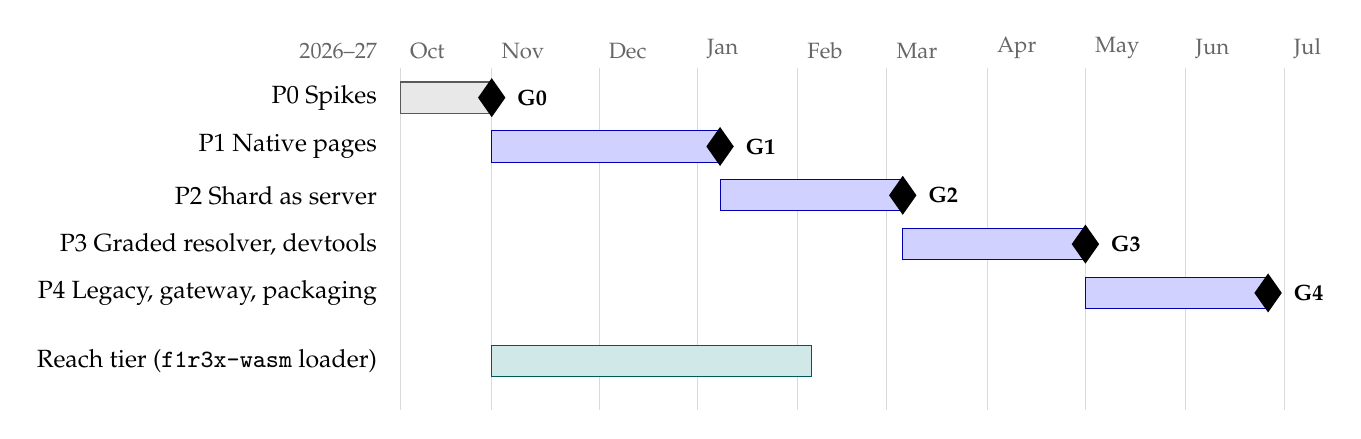
\begin{tikzpicture}[font=\small, x=0.29cm, y=0.62cm]
  % months: week offsets from 5 Oct 2026
  \foreach \w/\m in {0/Oct,4/Nov,8.7/Dec,13/Jan,17.4/Feb,21.3/Mar,25.7/Apr,30/May,34.4/Jun,38.7/Jul}{
    \draw[black!15] (\w,0.6) -- (\w,-6.4);
    \node[anchor=south west, font=\footnotesize, black!60] at (\w,0.6) {\m};
  }
  \node[anchor=south east, font=\footnotesize, black!60] at (-0.6,0.6) {2026--27};
  \newcommand{\phase}[5]{%
    \fill[#5!18] (#1,#2-0.32) rectangle (#1+#3,#2+0.32);
    \draw[#5!70!black] (#1,#2-0.32) rectangle (#1+#3,#2+0.32);
    \node[anchor=east, align=right] at (-0.6,#2) {#4};
  }
  \phase{0}{0}{4}{P0 Spikes}{gray}
  \phase{4}{-1}{10}{P1 Native pages}{blue}
  \phase{14}{-2}{8}{P2 Shard as server}{blue}
  \phase{22}{-3}{8}{P3 Graded resolver, devtools}{blue}
  \phase{30}{-4}{8}{P4 Legacy, gateway, packaging}{blue}
  \phase{4}{-5.4}{14}{Reach tier (\code{f1r3x-wasm} loader)}{teal}
  \foreach \x/\y/\g in {4/0/G0,14/-1/G1,22/-2/G2,30/-3/G3,38/-4/G4}{
    \fill[black] (\x,\y) ++(0,0.4) -- ++(0.6,-0.4) -- ++(-0.6,-0.4) -- ++(-0.6,0.4) -- cycle;
    \node[anchor=west, font=\footnotesize\bfseries] at (\x+0.7,\y) {\g};
  }
\end{tikzpicture}}
\caption{Indicative schedule from 5 October 2026, weeks to scale. Diamonds are gates;
their criteria are in the text.}
\label{fig:plan}
\end{figure}

\begin{description}[leftmargin=1.5em,style=nextline]
\item[P0 Spikes (4 weeks).] Link \code{blitz-dom} and the \Camp{} executive in one
  binary; mutate a document from a K1 program through a minimal bridge; measure the
  wasm size of the executive and the interpretation cost of a DOM-heavy workload in
  \code{b3ll0ws}. \emph{Gate G0}: a K1 program changes rendered text in a Blitz window,
  and the measurements are written down.
\item[P1 Native pages (10 weeks).] The page loader and the \code{.knf} format; free-name
  grounding through a stub broker; the DOM protocol; events as data with bubbling and
  default actions; frame-atomic commit; the Deterministic profile with event recording.
  \emph{Gate G1}: TodoMVC written in \fl{}, and a recorded session that replays
  identically.
\item[P2 Capabilities and the shard as server (8 weeks).] The capability broker
  with user prompts and revocable forwarders; \code{net} and \code{store}; the keystore
  and signed deploys; publishing and resolving \code{rho:serve} sites; hash-verified
  fetch of pages and blobs; key-bound sessions; the node inclusion-proof endpoint and the
  light-client check (Obligation~\ref{ob:proofs}), with quorum reads as the interim; the
  page meter. \emph{Gate G2}: a site published to a local three-validator shard loads
  through a deliberately hostile proxy that rewrites responses, and the browser refuses
  every rewritten resource; a session survives a replayed request without accepting it.
\item[P3 Graded resolver and devtools (8 weeks).] K2 on in the executive; the Graded
  oracle profile for the Viterbi, tropical and $\mathbb{R}_{\geq0}$ semirings; the
  fairness combinator; the ceiling check on drops; a devtools pane with replay, time
  travel and a live view of the space. \emph{Gate G3}: a page using a sampled clause
  replays identically from its log.
\item[P4 Legacy tab, gateway and packaging (8 weeks).] Servo in its own process
  behind one broker channel; the headless projection gateway with
  \code{Content-Digest}, signatures and links home; the session host with log anchoring;
  DNS and passkey bootstrap; the browser's own chrome rewritten as a \fl{} page;
  installers for macOS, Linux and Windows. \emph{Gate G4}: a public alpha.
\item[Reach tier (parallel, about 14 weeks at low intensity).] A loader and a
  host-DOM implementation of the same protocol over \code{f1r3x-wasm}, so that the
  G1 TodoMVC runs unchanged in stock browsers.
\end{description}

%======================================================================
\section{Risks, obligations and open decisions}\label{sec:risks}

\subsection{Risks}

\begin{center}
\begin{tabularx}{\linewidth}{@{}p{4.2cm}X@{}}
\toprule
Risk & Mitigation\\
\midrule
Blitz is beta with a small core team & Pin and vendor it; keep the bridge behind a trait
over the mutation interface so a Servo-layout or in-house tree could substitute; contribute
fixes upstream; the Stylo core is shared with Servo and Firefox\\
Interpreted normal forms are too slow for rich interfaces & The P0 measurement; the
\code{b3ll0ws} backend seam and the bytecode note's stated conditions for revisiting;
batching DOM messages per round\\
Fine-grained DOM messages flood the store & Structured fragments in \code{append} and
\code{replace}; coarse patch messages as an alternative (Decision~\ref{dec:granularity})\\
Text input, IME, forms and accessibility & Inherited from Blitz and AccessKit; tested
against the reach tier as an oracle\\
Graded clauses not yet in \Camp{} & K2 exists as a feature-gated level; P3 is scheduled
after the native path works without it\\
Legacy-tab compatibility & CEF fallback behind the same broker channel\\
\bottomrule
\end{tabularx}
\end{center}

\subsection{Obligations}

\begin{obligation}\label{ob:perf}
Measure, in P0, the frame-time cost of a representative interaction workload in
\code{b3ll0ws}, and state the threshold at which a compiled backend becomes necessary.
\end{obligation}

\begin{obligation}\label{ob:wasmdepth}
Decide, from measurement, whether running the executive as wasm inside the page process
is worth its cost as defence in depth.
\end{obligation}

\begin{obligation}\label{ob:replay}
Establish, through the \code{campf1r3-ispace} adapter's differential tests, whether
\Camp{} replays \code{rspace++} logs; client-side verification of shard results depends
on it.
\end{obligation}

\begin{obligation}\label{ob:graded}
Specify the Graded oracle profile in the \Camp{} specification (as a profile beside Free,
Deterministic and Replay), including how selections are logged for replay.
\end{obligation}

\begin{obligation}\label{ob:proto}
Write the DOM protocol as a specification, with its reply conventions, error names and
the attenuation rule, so the native bridge and the reach-tier bridge are tested against
one document.
\end{obligation}

\begin{obligation}\label{ob:proofs}
Add to \code{f1r3node-rust} an endpoint returning an inclusion proof from a registry
entry or data-at-name to a finalized block's \code{post\_state\_hash}, and specify the
browser's light-client check (validator signatures against a bonded-set checkpoint,
then the trie path).
\end{obligation}

\begin{obligation}\label{ob:hashes}
Fix one canonical hash for code stored in the registry: either the node records the
\Kind{} normal-form hash beside each entry, or the client re-normalises the returned term
and a differential test shows the two agree.
\end{obligation}

\begin{obligation}\label{ob:passkey}
Specify the passkey-to-session-key delegation, including the curve mismatch between
WebAuthn's usual P-256 and the node's deploy signatures.
\end{obligation}

\subsection{Open decisions}

\begin{decision}[Compilation in the browser]\label{dec:compile}
Ship only kernel normal forms in version~1, as proposed, or include the surface
\fl{} compiler so that pages can ship source?
\end{decision}

\begin{decision}[DOM message granularity]\label{dec:granularity}
Fine-grained messages per element, as proposed, or whole-subtree patches carried as
quoted processes, or both?
\end{decision}

\begin{decision}[The document language]
Keep HTML as the document language, or define it in the \fl{} DDL so that the document
is itself a term of a defined language, which the executive can already send and
receive? The first is compatible; the second is the more natural endpoint.
\end{decision}

\begin{decision}[Legacy engine]
Servo, as proposed, or CEF from the start, trading a large C++ dependency for
compatibility?
\end{decision}

\begin{decision}[Private sessions]\label{dec:privacy}
For confidential sessions, end-to-end encryption of payloads committed to the shard, or
private content kept on the session host with only hashes committed?
\end{decision}

\begin{decision}[Blob storage]
Where hash-addressed bytes live: a blob endpoint on the node, a separate content store run
by validators, third-party mirrors and CDNs, or all three?
\end{decision}

\begin{decision}[Repository and name]
A new repository under \code{F1R3FLY-io}, and a working name for the browser.
\end{decision}

%======================================================================
\begin{thebibliography}{99}\small

\bibitem{blitz} Dioxus Labs, \emph{Blitz: a modular HTML/CSS rendering engine},
  repository README (beta status, architecture, goals), accessed 28 September 2026.
  \url{https://github.com/DioxusLabs/blitz}

\bibitem{servolts} M.~Larabel, ``Servo browser engine making it easier for embedded
  use'' (crate publication and LTS policy; 0.1 LTS), \emph{Phoronix}, 13 April 2026.
  \url{https://www.phoronix.com/news/Servo-Embed-Crates-LTS}

\bibitem{servo05} M.~Larabel, ``Servo 0.5 released'', \emph{Phoronix}, 2026.
  \url{https://www.phoronix.com/news/Servo-0.5-Released}

\bibitem{electron} endoflife.date, \emph{Electron} (release cadence and support
  policy). \url{https://endoflife.date/electron}

\bibitem{cef} \emph{Chromium Embedded Framework}, Wikipedia, and the \code{cef} Rust
  crate. \url{https://en.wikipedia.org/wiki/Chromium_Embedded_Framework},
  \url{https://lib.rs/crates/cef}

\bibitem{atrium} J.~Asmar, ``From WKWebView to CEF: embedding Chromium in a Tauri
  app'', 22 May 2026. \url{https://getatrium.dev/blog/embedding-real-browser-tauri}

\bibitem{tauri} \emph{Tauri (software framework)}, Wikipedia.
  \url{https://en.wikipedia.org/wiki/Tauri_(software_framework)}

\bibitem{tauricef} Tauri pull request \#15980, \code{tauri-runtime-cef}, September
  2026. \url{https://github.com/tauri-apps/tauri/pull/15980}

\bibitem{ladybird} OpenReplay, ``Exploring Ladybird: the non-Chromium browser
  project'' (April 2026 newsletter figures, alpha roadmap).
  \url{https://blog.openreplay.com/fr/ladybird-navigateur-non-chromium/}

\bibitem{campf1r3} L.~G.~Meredith, \emph{\Camp{}}, \emph{\Kind{}}, and \emph{Bytecode,
  or the normal form?}, specifications in \code{publications/campf1r3}, September 2026;
  implementation in \code{F1R3FLY-io/campf1r3}.

\bibitem{gradedwhere} L.~G.~Meredith, \emph{Graded Where-Clauses}, and the choice-formulae
  note, \code{publications/fuzzyware} and \code{publications/choice-types}.

\bibitem{gradedpln} L.~G.~Meredith, \emph{Graded Where-Clauses over the Reals},
  \path{publications/fuzzyware/graded-where-pln.tex}.

\bibitem{gradedquantum} L.~G.~Meredith, \emph{Races Decided by the Born Rule},
  \path{publications/fuzzyware/graded-where-quantum-v6.tex}.

\end{thebibliography}

\end{document}
